\section{Methodology}
En este apartado se describen los métodos y procedimientos utilizados para la generación de reseñas de productos en plataformas de comercio electrónico mediante el uso de Modelos de Lenguaje de Gran Escala (LLMs). Se explican las etapas del proceso, desde la recopilación y preparación de datos hasta la evaluación de los modelos afinados. 
\\\\
Debido a que el \textit{dataset} ha sido generado desde cero, se detalla el procedimiento para la obtenci\'on y generación de los datos, así como la limpieza y estructuración de los mismos. Posteriormente, se describen las técnicas de afinación de modelos utilizadas, incluyendo la selección de hiperparámetros y métodos de optimización. Finalmente, se presentan las métricas de evaluación empleadas para analizar los resultados obtenidos.
\\\\
En la figura \ref{fig:MethodologyFlowchart} se muestra un diagrama de flujo que resume la metodología seguida en este trabajo. Se iniciar\'a explicando sobre la extracci\'on de datos, seguido por la preparaci\'on de los mismos, la afinaci\'on de los modelos y finalmente la evaluaci\'on de los resultados obtenidos.

\begin{figure}[H]
    \centering
    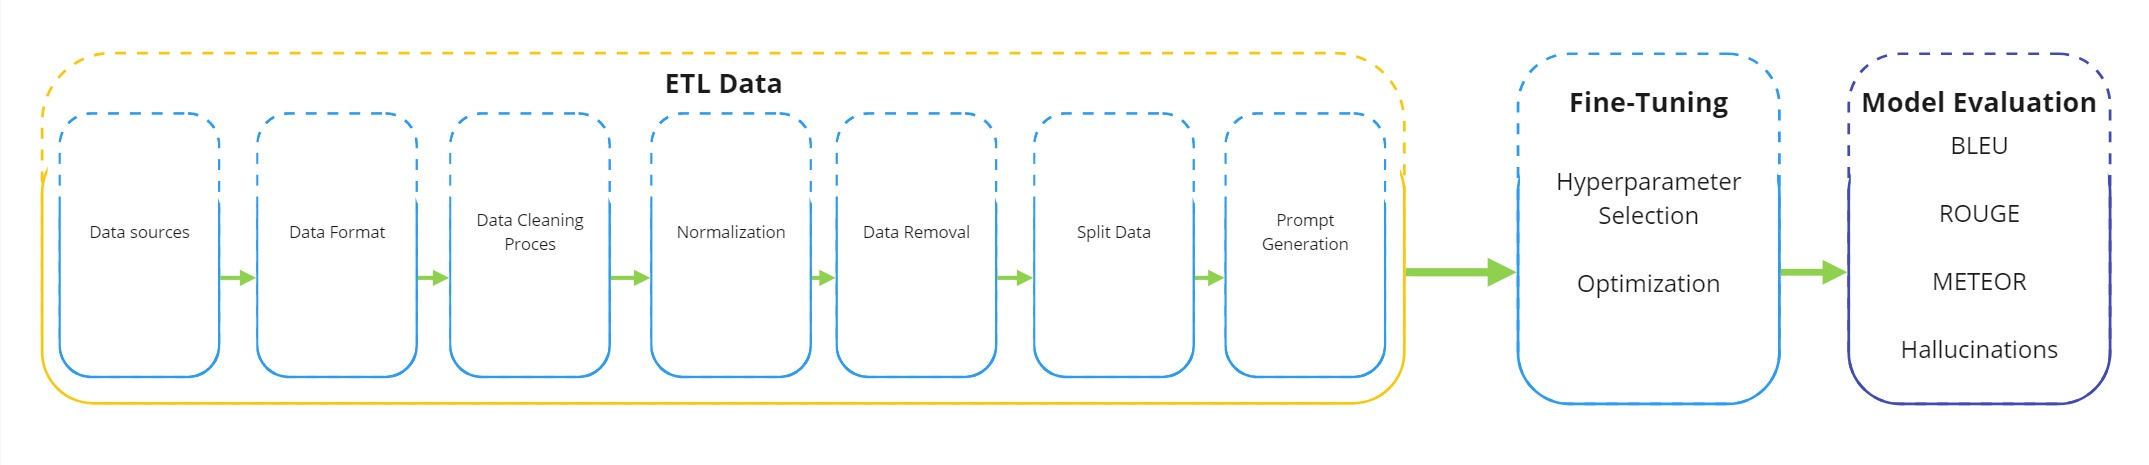
\includegraphics[width=12cm]{images/Methodology.jpg}
    \caption{Methodology Flowchart}
    \label{fig:MethodologyFlowchart}
\end{figure}